\documentclass[]{interact}
% Use Latin Modern fonts
\usepackage{lmodern}
\usepackage{float}
\usepackage{graphicx}
% Include algorithm2e for algorithm environment
\usepackage[ruled,vlined]{algorithm2e}
% To incorporate .eps illustrations using PDFLaTeX
\usepackage{epstopdf}
% Support for small, `sub' figures and tables
\usepackage[caption=false]{subfig}
% Citation support using natbib.sty
\usepackage[numbers,sort&compress]{natbib}
% Citation support using natbib.sty
\bibpunct[, ]{[}{]}{,}{n}{,}{,}
% Bibliography support using natbib.sty
\renewcommand\bibfont{\fontsize{10}{12}\selectfont}
% @ becomes a letter
\makeatletter
% Suppress spaces between citations using natbib.sty
\def\NAT@def@citea{\def\@citea{\NAT@separator}}
% @ becomes a symbol again
\makeatother
% Theorem-like structures provided by amsthm.sty
\theoremstyle{plain}
\newtheorem{theorem}{Theorem}[section]
\newtheorem{lemma}[theorem]{Lemma}
\newtheorem{corollary}[theorem]{Corollary}
\newtheorem{proposition}[theorem]{Proposition}
% 
\theoremstyle{definition}
\newtheorem{definition}[theorem]{Definition}
\newtheorem{example}[theorem]{Example}
%
\theoremstyle{remark}
\newtheorem{remark}{Remark}
\newtheorem{notation}{Notation}


\begin{document}


\articletype{RESEARCH ARTICLE}

\title{Optimized Data Partitioning for Parallel Sorting on Heterogeneous Distributed Systems using Linear Programming}

\author{
\name{Joeniño Cainday and Dr. Junar Landicho}
% TODO: thanks is on the template
% \thanks{CONTACT Joeniño Cainday. Email: caindayjoeninyo@gmail.com}
\affil{Department of Computer Science, University of Science and Technology of Southern Philippines, Cagayan De Oro City, Philippines}
}

\maketitle

\begin{abstract}
Do not read this as its just a placeholder. This research addresses the optimization of data partitioning for parallel computations in heterogeneous distributed systems, with the dual objective of minimizing financial expenditure and execution time. We develop a Mixed Integer Programming (MIP) model that incorporates critical system constraints including CPU speed, memory capacity, memory latency, network latency, and budget limitations. Our model replaces the heuristic partitioning phase of a parallel quicksort algorithm, which serves as our performance benchmark. Utilizing synthetic datasets representing both workload and node specifications, our simulations focus on pre-execution data partitioning decisions. The goal is to provide a framework for financial and time optimization within cloud computing environments, where efficient resource allocation and budget management are essential. Results demonstrate the effectiveness of our MIP-based approach in achieving improved load distribution and reduced runtime compared to traditional heuristics.
\end{abstract}

\begin{keywords}
Data Partitioning; Linear Programming; Heterogeneous Distributed Systems; Cost Optimization; Makespan Minimization
\end{keywords}

\section{Introduction}

The widespread adoption of cloud computing and serverless architectures has increased the importance of efficient resource allocation in distributed systems. This research addresses the challenge of statically partitioning data across heterogeneous computing environments, where nodes vary in processing speed, memory capacity, network latency, and monetary implications.

We formulate data partitioning as a Linear Programming (LP) problem aimed at minimizing execution time (makespan) while adhering to defined constraints. Our approach replaces traditional heuristic-based partitioning in parallel sorting algorithms with a novel LP model that captures comprehensive system characteristics to produce balanced, cost-aware data distributions. Our linear formulation allows polynomial-time solvability, providing optimal partitioning under linear constraints without incurring computational intractability.

\subsection{Background and Motivation}

Distributed computing enables parallel processing of large-scale datasets across multiple nodes. However, in heterogeneous systems with diverse computational capabilities, simplistic data partitioning strategies often result in load imbalances and inefficient resource utilization[48]. Common approaches like uniform distribution or partitioning based solely on heuristics typically fail to consider system compositions in cloud environments.

Cloud computing introduces new complexities to data partitioning. These environments offer flexibility with pay-as-you-go pricing models where computing resources are available on demand[5]. This necessitates re-evaluating traditional partitioning methodologies to explicitly consider economic factors alongside performance metrics. Effective strategies must balance high performance with budget limitations—minimizing both computational time and overall expenditure for cloud resource utilization. 

While Monga and Lodhi[53] demonstrated benefits of heterogeneity-aware allocation, their model primarily considered CPU speed alone. Our work introduces a more sophisticated LP-based model that integrates multiple system attributes to achieve globally optimized data distributions, providing a more realistic and budget-conscious approach to optimized data processing.

\subsection{Cost Considerations in Heterogeneous Distributed Systems}

In this context, cost refers to the pricing of cloud compute nodes. While higher-priced instances often imply better performance, this is not guaranteed, as pricing and performance can vary across vendors. Each node has attributes including processing speed, memory capacity, network characteristics, and pricing models inspired by real cloud offerings, reflecting typical variations in heterogeneous cloud deployments.

Allocating data across heterogeneous resources inherently involves performance-cost tradeoffs[48]. Balancing processing time with financial implications when assigning datasets to different machines is critical. Effective data partitioning can significantly reduce both runtime and monetary cost, while suboptimal partitioning leads to inflated expenses or resource limitations like memory overflows. 

This paper specifically addresses statically partitioning large synthetic datasets before executing parallel sorting across simulated heterogeneous environments. Our primary objective is to minimize the overall execution time (makespan) while ensuring we satisfy the defined constraints. As a secondary objective, we aim to identify the most cost-effective solution with an equivalent makespan, using a lexicographic optimization approach. The controlled synthetic environment enables repeatable experiments independent of real-world cloud variability.

Linear programming offers a powerful and tractable mathematical framework for such optimization problems, especially when:
\begin{itemize}
    \item Data volumes are represented as continuous variables;
    \item Constraints and objectives remain linear;
    \item No integer or combinatorial decisions are involved;
\end{itemize}
This allows the use of efficient solvers that provide globally optimal solutions in polynomial time [57]. By leveraging LP, we avoid the complexity of NP-hard integer-based scheduling, while still capturing key system characteristics through continuous modeling of load, speed, and cost.

\subsection{Research Contributions}

This paper contributes the following:
\begin{enumerate}
    \item A linear programming (LP) formulation for initial data partitioning in parallel quicksort on heterogeneous systems;
    \item An integration of the LP model into an existing heterogeneous sorting framework;
    \item A performance evaluation using synthetic datasets with extended metrics;
    \item A reproducible experimental setup and discussion of directions for future work.
\end{enumerate}

\section{Related Work}
\label{sec:related_work}
Heterogeneous scheduling and data allocation have been studied in various contexts. For instance,[48] considered dataset allocation across geo-distributed clouds with two objectives (processing time and cost). They formulated a linear program to place data blocks on VMs to minimize a weighted sum of time and cost, demonstrating Pareto trade-offs. Similarly,[49] used a linear model for data assignment in a hybrid heterogeneous processing environment. These works focus on resource assignment rather than within-job data partitioning, but they highlight the utility of mathematical programming for cloud cost-performance optimization.

Classic scheduling theory demonstrates that minimizing makespan on unrelated machines is NP-hard when tasks must be assigned discretely[50]. However, in our case, we model data volumes as continuous variables without requiring integer decision variables. This places our problem within the class of linear programs, which are solvable in polynomial time using interior-point methods or simplex-based solvers [57]. Thus, our static data partitioning model, while inspired by hard scheduling problems, does not inherit their computational complexity due to the absence of discrete allocation and the use of continuous variables.

In the domain of parallel sorting, many algorithms assume a homogeneous machine model. For instance, Parallel Sorting by Regular Sampling (PSRS) chooses pivots to create equally-sized partitions[51], and typical benchmarks use randomly-generated data with uniform or other distributions. These benchmarks (e.g., uniform 32-bit integer inputs) guide our synthetic data choices. However, PSRS and related methods do not account for cost or heterogeneous speeds.

In big-data systems like Spark, dynamic partitioning and scheduling algorithms have been proposed. For example,[52] developed a dynamic partitioning strategy for intermediate Spark data to mitigate skew, and a greedy scheduling method that considers node speed. They find that balanced partitioning significantly lowers completion time. Our work differs by focusing on static initial partitioning with explicit cost metrics, rather than in-job rebalancing. To the best of our knowledge, prior work has not explicitly applied linear programming to cost-aware static data partitioning in heterogeneous cloud sort workloads.

We build upon the model proposed by Monga and Lodhi[53], which partitions data across heterogeneous nodes based on CPU performance to balance load during parallel sorting. However, their approach does not consider critical real-world factors such as network latency or resource cost—key limitations in cloud and serverless settings. Moreover, their method performs initial local sorting and sampling before defining data ranges, which can lead to uneven memory usage and load imbalance during the redistribution phase.




% This section presents our approach combining Mixed Integer Programming (MIP) for optimal data partitioning with the parallel Quicksort algorithm proposed by Monga and Lodhi [53].

\section{Problem Formulation}

We now formalize the partitioning problem based on the system characteristics introduced in Section 1.3. To ensure full control over system parameters and facilitate reproducibility, we operate within a synthetic environment. Each node is defined by parameters such as processing speed, memory capacity, network latency, bandwidth, and cost, inspired by real-world cloud configurations (e.g., AWS, GCP). This abstraction enables rigorous evaluation of partitioning strategies without relying on live infrastructure.

\subsection{System Model}

We partition the dataset into contiguous blocks of size $d$, assigning each block to a unique node. Consider a heterogeneous cluster with $N$ nodes, where each node $i$ is characterized by the following parameters:

\begin{itemize}
    \item $d_i$: Assigned data volume (in units of $d$)
    \item $r_i$: Processing rate (in $d/t$ — data units per time unit)
    \item $m_i$: Maximum data volume the node can handle at once (in units of $d$)
    \item $\ell_i$: Network latency (in time units $t$)
    \item $b_i$: Network bandwidth (in $d/t$ — data units per time unit)
    \item $u_i$: Usage billing rate (in $c/t$ — cost units per time unit)
\end{itemize}

The units above are illustrative and can be adapted depending on context. For instance, processing speed $r$ may be measured in records/ms, memory $m$ in megabytes (MB), and cost $u$ in USD/hour. In this work, we use normalized or synthetic units to model relative performance and cost differences between nodes, without binding the system to a specific infrastructure or currency.

\subsection{Derived Parameters}
We derive additional parameters from the node characteristics to facilitate the MIP formulation:

\subsubsection{Processing Time}
\begin{equation}
    x_i = \frac{d_i}{r_i}
\end{equation}
where $x_i$ is the time required by node $i$ to process its assigned data volume $d_i$.

\subsubsection{Transfer Time}
\begin{equation}
    y_i = \ell_i + \frac{d_i}{b_i}
\end{equation}
where $y_i$ is the communication overhead for node $i$, computed from latency $\ell_i$ and bandwidth $b_i$.

\subsubsection{Total Cost}
\begin{equation}
    w = \sum_{i=1}^N u_i \cdot x_i
\end{equation}
where $w$ denotes the cumulative cost of utilizing all selected nodes.

\subsection{Optimization Objectives}
The primary objective of our MIP model is to minimize the total execution time (makespan) of the parallel sorting process. This ensures that the overall completion time is minimized, taking into account both computation and communication overheads. Formally, the primary objective is defined as:
\begin{equation}
    \min z = \max_{i=1}^N (x_i + y_i)
\end{equation}
where $z$ represents the maximum time taken by any node $i$ to complete its assigned data processing and communication tasks. This formulation captures the makespan of the entire parallel sorting operation, ensuring that the slowest node determines the overall completion time. In addition to minimizing makespan, we aim to choose the most cost-effective solution among equivalent combinations. To achieve this, we introduce a secondary objective that minimizes the total financial expenditure. This is incorporated into the model using a lexicographic optimization approach:
\begin{equation}
    \min \ z + \varepsilon \cdot w
\end{equation}
In this formulation, $w$ represents the cumulative cost of utilizing the selected nodes, and $\varepsilon$ is set to a negligible value (e.g., $10^{-6}$) to prioritize makespan minimization while breaking ties in favor of cost efficiency. This approach ensures that among solutions with equivalent makespan, the one with the lowest cost is selected.

\subsection{Constraint Definitions}

The proposed LP model is subject to several constraints that reflect system limitations and ensure a feasible allocation of data across nodes. These constraints incorporate resource boundaries (e.g., memory and budget), performance considerations (e.g., makespan), and completeness of the partitioning scheme.

\subsubsection{Makespan Constraint}
\begin{equation}
    z \geq \frac{d_i}{r_i} + \ell_i + \frac{d_i}{b_i} \quad \forall i \in \{1, \ldots, N\}
\end{equation}
This constraint ensures that the total execution time, represented by the variable $z$, is at least as large as the time taken by any individual node $i$ to both process its assigned data and transfer it to the next stage. It combines computation time $\frac{d_i}{r_i}$ with communication latency $\ell_i$ and data transfer time $\frac{d_i}{b_i}$.

\subsubsection{Memory Constraint}
\begin{equation}
    d_i \leq m_i \quad \forall i \in \{1, \ldots, N\}
\end{equation}
Each node has a limited memory capacity $m_i$, and this constraint ensures that the volume of data $d_i$ assigned to node $i$ does not exceed its available memory.

\subsubsection{Coverage Constraint}
\begin{equation}
    \sum_{i=1}^{N} d_i = D
\end{equation}
This constraint enforces full data allocation: the entire dataset of size $D$ must be partitioned and distributed among the $N$ available nodes without omission or duplication.

\subsubsection{Non-negativity Constraint}
\begin{equation}
    d_i \geq 0 \quad \forall i \in \{1, \ldots, N\}
\end{equation}
This standard constraint ensures that each node receives a non-negative volume of data, reflecting the physical impossibility of assigning negative quantities.


\subsubsection{Budget Constraint (Optional)}
\begin{equation}
    0 \leq \sum_{i=1}^{N} u_i \cdot d_i \leq B
\end{equation}
In addition to node-specific parameters, we optionally define a user-defined input $B$, representing the maximum allowable expenditure. This parameter must be a non-negative number, with a default value of $0$. Including this constraint models scenarios where financial limitations must be respected.











\section{Heterogeneous PSRS (Baseline Algorithm)}

This is the model of Monga and Lodhi [53] which we will use as a baseline. The algorithm is designed to sort a list of items using multiple workers, each with different speeds.

\subsection{Pseudocode}

\begin{algorithm}[H]
\caption{Heterogeneous PSRS (Baseline Algorithm)}
\SetKwInput{KwInput}{Inputs}
\KwInput{
    \begin{itemize}
        \item $data$: Input data to be sorted
        \item $n$: Total number of data items
        \item $p$: Number of processors
        \item $perf[0 \dots p-1]$: Relative performance of each processor
    \end{itemize}
}
\SetKwInput{KwOutput}{Output}
\KwOutput{
    \begin{itemize}
        \item Sorted data
    \end{itemize}
}

\textbf{Phase 1: Local Sorting and Sampling} \\
\For{each processor $i$}{
    $size_i = \frac{n \cdot perf[i]}{\sum perf}$ \\
    Assign $size_i$ items to processor $i$ \\
    Processor $i$ performs sequential quicksort on its local data \\
    Select $L = (p - 1) \cdot perf[i]$ samples from local sorted data \\
    Send samples to the designated coordinator
}

\textbf{Phase 2: Pivot Selection} \\
Designated coordinator gathers and sorts all samples \\
Selects $p - 1$ global pivots and broadcasts them to all processors

\textbf{Phase 3: Data Redistribution} \\
\For{each processor}{
    Partition local data using global pivots \\
    Send partitioned data to corresponding processors \\
    Retain the portion corresponding to its final range
}

\textbf{Phase 4: Final Sorting and Merge} \\
Each processor sorts its final local data \\
Coordinator concatenates all sorted segments for final output
\end{algorithm}

\subsection{Limitations}

The Heterogeneous PSRS algorithm by Monga and Lodhi[53] effectively distributes sorting tasks across processors with varying speeds but has notable inefficiencies. Its local sorting phase precedes global partitioning, often leading to imbalanced data redistribution, where some nodes receive disproportionately larger portions. This imbalance increases memory usage and processing delays. Additionally, the algorithm overlooks communication costs and network latency, critical factors in distributed and cloud-based systems. These limitations highlight the need for a more adaptive approach that integrates performance and cost considerations when assigning data ranges.






\section{LP-Guided Sorting (Proposed Algorithm)}

We propose a modified algorithm that replaces the sampling and redistribution stages with a LP formulation that statically partitions the global key range across heterogeneous distributed nodes.

\subsection{Bucket Assignment}

Given the total dataset size $D$ and a heterogeneous set of $N$ nodes with parameters $(r_i, m_i, \ell_i, b_i, u_i)$, we solve the MIP formulation (Section~\ref{sec:methodology}) to compute optimal partition sizes $d_i$ such that:

\begin{itemize}
    \item Processing time is balanced according to each node's capability
    \item Communication and processing costs are minimized
    \item Constraints on memory, load, and budget are respected
\end{itemize}

Once $d_i$ values are determined, each node is assigned a fixed key range. For example (illustrative only):

\begin{center}
\footnotesize
\renewcommand{\arraystretch}{1.5} % Adjust the row height
\begin{tabular}{|p{6.7cm}|p{6.7cm}|}
\hline
\textbf{Worker} & \textbf{Percentage of Total Data} \\
\hline
A (4x speed) & 50\% \\
\hline
B (3x speed) & 30\% \\
\hline
C (2x speed) & 20\% \\
\hline
\end{tabular}
\end{center}

\subsection{Merge Strategies}

\begin{table}[H]
\centering
\renewcommand{\arraystretch}{1.5} % Adjust the row height
\footnotesize
\begin{tabular}{|p{3cm}|p{5cm}|p{5cm}|}
\hline
\textbf{Aspect} & \textbf{Option A: Block Merge (Centralized Bucketing)} & \textbf{Option B: Coordinated Min-Max Pop (Asynchronous Routing)} \\ \hline
Data Handling & Each node returns a fully sorted block corresponding to a unique key range & Coordinator continuously requests the current min and max from each node's local sorted data \\ \hline
Merge Strategy & Coordinator performs a two-ended merge by popping global min and max from the node outputs & Dynamically merges results by selecting the global min and max across all nodes \\ \hline
Efficiency & Efficient for well-partitioned data; avoids re-querying nodes & Suitable when node outputs are fragmented or partially overlapping \\ \hline
Memory Usage & Requires all blocks to be received and held in memory before merging & Lower memory usage as data is processed dynamically \\ \hline
Coordination Overhead & Minimal; relies on pre-sorted blocks & Higher coordination overhead; increases latency and total merge time \\ \hline
\end{tabular}
\caption{Comparison of Merge Strategies}
\end{table}


\subsection{Pseudocode}

\begin{algorithm}[H]
\caption{LP-Guided Hybrid (Proposed Algorithm)}

\SetKwInput{KwInput}{Inputs}
\KwInput{
    \begin{itemize}
        \item $D$: Total dataset
        \item $N$: Number of nodes
        \item $r_i$: Processing rate of node $i$
        \item $m_i$: Memory capacity of node $i$
        \item $b_i$: Network bandwidth of node $i$
        \item $\ell_i$: Network latency of node $i$
        \item $u_i$: Usage cost rate of node $i$
    \end{itemize}
}

\SetKwInput{KwOutput}{Output}
\KwOutput{
    \begin{itemize}
        \item Sorted dataset
    \end{itemize}
}

\textbf{Phase 1: Static Partitioning} \\
Solve LP to determine proportion $p_i$ of data that node $i$ should process, where $\sum p_i = 1$ \\
Compute data volume per node: $d_i = p_i \cdot |D|$

\textbf{Phase 2: Block Distribution} \\
For each node $i$, calculate how many items it should receive by multiplying its proportion $p_i$ with the total number of items $|D|$, then rounding down: $\text{floor}(p_i \cdot |D|)$ \\
Set starting index $c_0 = 0$ and compute cut points $c_i$ by adding up the sizes \\
\For{each node $i$ from $1$ to $N$}{
    Distribute subarray $D[c_{i-1} : c_i]$ to node $i$
}


\textbf{Phase 3: Local Sorting} \\
\For{each node $i$}{
    Sort received data using sequential quicksort
}

\textbf{Phase 4: Final Merge} \\

\textbf{Option A: Centralized Block} \\
Let $S_1, S_2, \ldots, S_N$ be the sorted blocks received from each node \\
Initialize a double-ended queue: $\texttt{merged\_sorted} \leftarrow$ empty deque \\

\While{any $S_i$ is non-empty}{
    Identify the global minimum and maximum from heads and tails of non-empty $S_i$ \\
    Pop the global min and append to the \textbf{left}, max to the \textbf{right} of $\texttt{merged\_sorted}$
}

\Return{$\texttt{merged\_sorted}$}

\vspace{2mm}

\textbf{Option B: Coordinated Min-Max Pop} \\
Initialize a double-ended queue: $\texttt{merged\_sorted} \leftarrow$ empty deque \\
Let each node expose head and tail of its local sorted buffer on request \\

\While{total number of popped elements $< |D|$}{
    \ForEach{node $i$}{
        Send $h_i$ and $t_i$ (head and tail) to coordinator
    }
    Coordinator selects global min and max from all $h_i$, $t_i$ \\
    Source nodes pop their respective elements \\
    Append global min to \textbf{left}, global max to \textbf{right} of $\texttt{merged\_sorted}$
}

\Return{$\texttt{merged\_sorted}$}

\end{algorithm}
    






% Starting the section for theoretical complexity analysis
\section{Theoretical Complexity Analysis}

% Introducing the complexity analysis
A rigorous complexity analysis highlights the theoretical advantages of our LP-guided approach over the baseline PSRS algorithm, particularly in heterogeneous distributed nodes.

% Subsection for the baseline algorithm
\subsection{Baseline Algorithm}

% Subsubsection for time complexity
\subsubsection{Time Complexity}
The original Heterogeneous PSRS algorithm involves four distinct phases, each contributing to the overall time complexity:

% Paragraph for Phase 1: Local Sorting and Sampling
\paragraph{Phase 1: Local Sorting and Sampling} 
Each of the $N$ nodes sorts its local data of size $O(n/N)$ on average, taking $O\left(\frac{n}{N} \log \frac{n}{N}\right)$ time using quicksort. Sampling takes $O(N)$ time per node. The communication of samples to the coordinator takes $O(N^2)$ in the worst case if all nodes send their $O(N)$ samples sequentially. Thus, this phase has an average time complexity of $O\left(\frac{n}{N} \log \frac{n}{N} + N^2\right)$.

% Paragraph for Phase 2: Pivot Selection
\paragraph{Phase 2: Pivot Selection}
The coordinator sorts $O(N^2)$ samples, which takes $O(N^2 \log N^2) = O(N^2 \log N)$ time. Broadcasting the $N - 1$ pivots to all $N$ nodes takes $O(N)$ time in parallel or $O(N^2)$ sequentially.

% Paragraph for Phase 3: Data Redistribution
\paragraph{Phase 3: Data Redistribution} Each node partitions its $O(n/N)$ local data using $N - 1$ pivots, which takes $O(n/N \cdot N) = O(n)$ in the worst case if the pivots are poorly chosen. The redistribution of data among nodes can take up to $O(n)$ in the worst-case scenario where one node receives almost all the data.

% Paragraph for Phase 4: Final Sorting and Merge
\paragraph{Phase 4: Final Sorting and Merge} Each node sorts its received data, which can be up to $O(n)$ in the worst case, leading to $O(n \log n)$ for a single node if load balancing is poor. The coordinator then merges the $N$ sorted segments, which takes $O(n)$ time.

% Paragraph for overall complexity
\paragraph{Overall Complexity} 
The PSRS algorithm executes in four distinct phases: local sorting and sampling, pivot selection, data redistribution, and final sorting or merging. Combining these phases, the average-case time complexity of the original PSRS algorithm is dominated by the local sorting and pivot selection, yielding

\begin{equation}
    \mathcal{O}\left( \underbrace{\frac{n}{N} \log \frac{n}{N}}_{\text{local sorting}} + \underbrace{N^2 \log N}_{\text{pivot selection}} + \underbrace{n}_{\text{redistribution}} \right)
\end{equation}
Under ideal load balancing and when \(N \ll n\), this simplifies to:
\begin{equation}
    \mathcal{O}\left( \underbrace{\frac{n \log n}{N}}_{\text{local sorting}} + \underbrace{N^2 \log N}_{\text{pivot selection}} \right) \quad \text{(since \(\log \frac{n}{N} \approx \log n\) for \(N \ll n\))}
\end{equation}
However, due to dynamic pivot selection and load imbalance:
\begin{itemize}
     \item If one node is assigned a disproportionately large portion of the data, the worst-case time complexity becomes:
        \begin{equation}
            \mathcal{O}\left( \underbrace{n \log n}_{\text{sorting dominated by the largest partition}} \right)
        \end{equation}
        \item If the local sorting algorithm performs poorly on specific input patterns (e.g., quicksort with highly unbalanced partitions):
        \begin{equation}
            \mathcal{O}\left( \underbrace{n^2}_{\text{quadratic worst-case sorting due to poor partitioning}} \right)
        \end{equation}
\end{itemize}

% Subsubsection for space complexity
\subsubsection{Space Complexity}
For space complexity, the PSRS algorithm requires local storage for each node to store its assigned data, which is $O(n/N)$ on average. 

\paragraph{Phase 1: Local Sorting and Sampling} 
During the local sorting and sampling phase, each node stores its assigned data locally, requiring $O(n/N)$ space. Additionally, each node generates $O(N)$ samples, which are sent to the coordinator. The coordinator stores $O(N^2)$ samples in total, as it collects $O(N)$ samples from each of the $N$ nodes.

\paragraph{Phase 2: Pivot Selection} 
In the pivot selection phase, the coordinator sorts the collected $O(N^2)$ samples. This requires $O(N^2)$ space for storing and processing the samples. The pivots themselves, $N - 1$ in number, require negligible additional space.

\paragraph{Phase 3: Data Redistribution} 
During data redistribution, nodes may need temporary buffers to hold data being sent or received. These buffers can be up to $O(n/N)$ in size per node, depending on the volume of data being exchanged.

\paragraph{Phase 4: Final Sorting and Merge} 
In the final sorting and merge phase, each node holds a sorted segment of approximately $O(n/N)$. The coordinator may require additional space to merge the sorted segments, but this is typically $O(n)$ as it processes the entire dataset.

\paragraph{Overall Space Complexity} 
The total space complexity of the PSRS algorithm is $O(n)$, as the total data is partitioned and stored across the nodes. The coordinator requires additional space for the samples, $O(N^2)$, which is negligible compared to the total data size for large $n$.

% Subsection for the proposed algorithm
\subsection{Proposed Algorithm}
For the LP-guided algorithm, the process is significantly streamlined.

% Subsubsection for time complexity
\subsubsection{Time Complexity}

\paragraph{Phase 1: Static Partitioning}
This is solved once as a precomputation step. The complexity of solving a Linear Programming problem is polynomial, typically handled by efficient algorithms like the interior-point method or simplex method. For practical LP solvers, the complexity is often approximated as $O(N^3)$, where $N$ is the number of nodes, based on the number of variables (proportional to $N$) and constraints (also proportional to $N$). 

Although the constraint matrix of a linear program has \(O(N^2)\) entries, solving the LP involves more than just accessing these entries. Matrix operations such as factorization or inversion generally take \(O(N^3)\) time [57]. While sparsity can reduce this in practice, we conservatively estimate the complexity as $O(N^3)$. This is a one-time overhead, and for a fixed number of nodes $N$, it becomes negligible over repeated runs.

\paragraph{Phase 2: Data Distribution}
Since the assignment is static and precomputed, each node directly receives its designated data block without coordination overhead or routing logic. The data is assumed to be globally addressable or pre-divided based on offsets, so the coordinator does not mediate or relay data. This results in a linear time complexity for distribution $O(n)$ as each of the $n$ items is sent directly to its assigned node.

\paragraph{Phase 3: Local Sorting}
Each of the $N$ nodes sorts its assigned partition of size $d_i$. Since the LP aims to balance the workload, we expect $d_i \approx O(n/N)$. The sorting time per node is $O\left(\frac{n}{N} \log \frac{n}{N}\right)$. With parallel execution, the overall sorting time remains $O\left(\frac{n}{N} \log \frac{n}{N}\right)$.

\paragraph{Phase 4: Final Merge}
Both options use a coordinated merge phase where the coordinator retrieves the global minimum and maximum elements in each round. This requires scanning $N$ candidates per iteration, with $n/2$ iterations in total (since two items are merged per round), yielding a worst-case time complexity of $O(nN)$ for the merge. This step is optional if a distributed sorted output is acceptable.

\paragraph{Overall Complexity}
With the updated distribution phase, the total time complexity becomes:

\begin{equation}
    O\left( 
        \underbrace{N^3}_{\text{LP solve}} 
        + \underbrace{n}_{\text{distribution}} 
        + \underbrace{\frac{n}{N} \log \frac{n}{N}}_{\text{local sort}} 
        + \underbrace{nN}_{\text{merge}}
    \right)
\end{equation}

This streamlined model avoids the intermediate routing layer and central buffers entirely, improving both runtime and memory efficiency. When $N \ll n$, this simplifies to:

\begin{equation}
    O\left( 
        \underbrace{nN}_{\text{merge}} 
        + \underbrace{\frac{n}{N} \log \frac{n}{N}}_{\text{local sort}} 
    \right)
\end{equation}

amortizing the $O(N^3)$ LP cost over repeated executions.

\subsubsection{Space Complexity}
Each node stores only its assigned partition of size $d_i$, where $\sum d_i = n$, resulting in a total distributed memory usage of $O(n)$.

\paragraph{Phase 1: Static Partitioning}
The LP solver still consumes $O(N^2)$ space for storing the constraint matrix and internal buffers. This space is allocated once during initialization and reused across multiple executions.

\paragraph{Phase 2: Data Distribution}
With direct data assignment, no intermediate data structures are needed at the coordinator. Each item is sent directly to its destination node without temporary storage. Thus, the coordinator’s memory usage is reduced to only managing lightweight metadata (e.g., offsets or boundaries), which requires $O(N)$ space.

\paragraph{Phase 3: Local Sorting}
Each node performs an in-place sort on its local partition. Since no additional structures are required beyond the input array and constant auxiliary space for the sorting algorithm (e.g., quicksort or heapsort), the space complexity remains $O\left(\frac{n}{N}\right)$ per node. The total space across all nodes is still $O(n)$.

\paragraph{Phase 4: Final Merge}
The coordinated merge step requires the coordinator to keep track of one active element (or pointer) per node, resulting in $O(N)$ memory overhead. Optionally, if streaming is not used, the coordinator may need to buffer the entire merged result, requiring an additional $O(n)$ space.

\paragraph{Overall Space Usage}
\begin{itemize}
    \item LP solver and metadata: $O(N^2)$ at initialization.
    \item Total data storage: $O(n)$, distributed across $N$ nodes.
    \item Merge coordination: $O(N)$ for pointers; optionally $O(n)$ for buffering.
\end{itemize}




% Updated Formal Complexity Comparison Table
\subsection{Complexity Comparison}
In this section, we formally analyze and compare the time complexity of the baseline PSRS algorithm and the proposed LP-guided algorithm, incorporating both Option A and Option B for data distribution. The analysis emphasizes both average-case behavior and worst-case scenarios under heterogeneous processing environments.


\begin{table}[H]
\centering
\footnotesize
\renewcommand{\arraystretch}{1.5} % Adjust the row height
\begin{tabular}{|p{3.7cm}|p{4cm}|p{5.4cm}|}
\hline
\textbf{Algorithm} & \textbf{Average Case} & \textbf{Worst Case} \\ \hline
PSRS & $O\left(\frac{n \log n}{p} + p^2 \log p\right)$ & $O(n \log n)$ \\ \hline
LP-guided & $O(n + \frac{n}{N} \log \frac{n}{N} + nN)$ & $O(N^3 + n + \frac{n}{N} \log \frac{n}{N} + nN)$ \\ \hline
\end{tabular}
\caption{Time Complexity Comparison (Average vs Worst Case)}
\end{table}

\begin{table}[h]
\centering
\footnotesize
\renewcommand{\arraystretch}{1.5} % Adjust the row height
\begin{tabular}{|p{4.35cm}|p{4.35cm}|p{4.35cm}|}
\hline
\textbf{Algorithm} & \textbf{Average Case} & \textbf{Worst Case} \\
\hline
PSRS (Baseline) & $O(n)$ & $O(n)$ \\
\hline
LP-guided (Option A) & $O(n)$ & $O(2n + N^2)$ \\
\hline
LP-guided (Option B) & $O(n)$ & $O(n + N^2)$ \\
\hline
\end{tabular}
\caption{Space Complexity Comparison (Average vs Worst Case)}
\end{table}


% \begin{figure}[h]
%     \centering
%     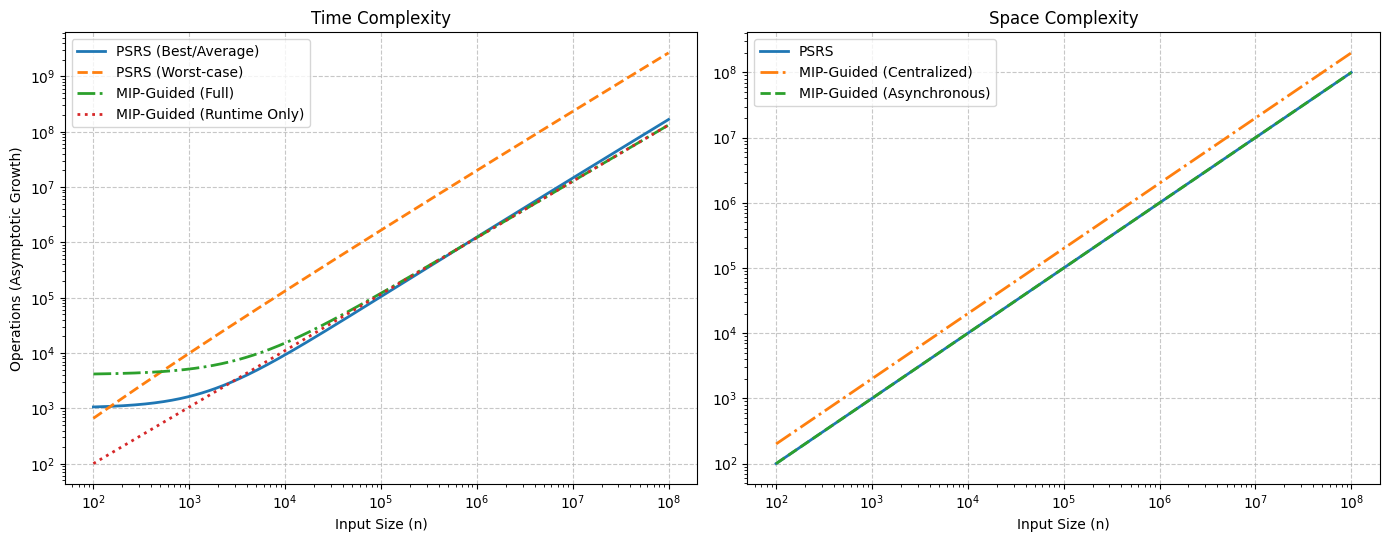
\includegraphics[width=1\textwidth]{graph-complexity.png}
%     \caption{Complexity Comparison Graph}
%     \label{fig:example}
% \end{figure}

    
\begin{table}[H]
\footnotesize
\renewcommand{\arraystretch}{1.5} % Adjust the row height
\begin{tabular}{|p{3cm}|p{5cm}|p{5cm}|}
\hline
\textbf{Aspect} & \textbf{PSRS} & \textbf{LP-Guided} \\
\hline
Load Balancing & Data-dependent and dynamic, prone to imbalance & Statically balanced using node profiles \\
\hline
Synchronization & Multiple barriers: sampling, pivoting, merging & Minimal, only at merge (if needed) \\
\hline
Communication Overhead & $O(p^2)$ (samples), $O(n)$ (data) & $O(n)$ (initial only) \\
\hline
Preprocessing & None & One-time $O(N^3)$ for LP \\
\hline
Memory Usage & Prone to imbalance due to uneven partition sizes & Evenly balanced partitions based on LP solution \\
\hline
Worst-case & $O(n \log n)$ & Consistently balanced, better in heterogeneity \\
\hline
\end{tabular}
\caption{Performance Factors Comparison}
\end{table}

The LP-guided algorithm offers clear advantages over PSRS in terms of scalability, memory balance, and load distribution. By eliminating runtime sampling and pivot-based partitioning, LP-guided minimizes both load and memory imbalance as well as communication overhead, making it particularly suitable for heterogeneous systems.

\textbf{Time complexity:}
\begin{itemize}
    \item PSRS relies on dynamic sampling and pivot selection, which can lead to inefficiencies on large systems with many nodes.
    \item LP-guided approaches require preprocessing but offer more consistent performance, especially in repeated or large-scale sorting tasks.
\end{itemize}

\textbf{Space complexity:}
\begin{itemize}
    \item PSRS is memory-efficient on average but may suffer from \textit{memory imbalance} if partition sizes vary significantly due to skewed data.
    \item LP-guided approaches incur preprocessing overhead but provide \textit{deterministic partitioning}, leading to better memory balance and overall scalability.
\end{itemize}

Overall, LP-guided algorithms are better suited for scenarios requiring repeated sorts or large datasets on heterogeneous constraints. PSRS remains viable for simpler, homogeneous setups with fewer nodes and lower memory pressure.


\section{Experimental Setup}

To evaluate the proposed LP-Guided Hybrid Sorting algorithm, we developed a simulation environment in Python that emulates a distributed system comprising heterogeneous artificial nodes. Each node is modeled with distinct computational and network characteristics to reflect real-world cloud or edge environments. Our setup draws inspiration from prior work, such as Monga and Lodhi’s evaluation on a heterogeneous cluster of UltraSPARC processors, while extending the model with scalable simulation and optimization capabilities.


For each experiment, we perform an initial warm-up run to allow the LP solver and runtime components to initialize. The LP component is implemented using Google's OR-Tools, which introduces a slight startup cost during the first invocation. We then execute three measured runs and report the average execution time. This ensures that reported results reflect the algorithm's steady-state performance, excluding one-time overhead.


Nodes execute local sorts on subarrays and participate in global merges, coordinated either centrally or collaboratively. Resource constraints are enforced strictly throughout the simulation.

\subsection{Dataset}
We generated synthetic datasets $D$ of uniformly distributed integers with sizes ranging from $10^3$ to $10^6$ elements. Each dataset is randomly shuffled before processing. Additionally, to simulate skewed distributions akin to Monga and Lodhi’s setup, we tested with datasets containing concentrated ranges of values interspersed with random values.




\subsection{Environment}

We evaluate scalability and heterogeneity by simulating clusters of three sizes: $N=3$, $6$, and $12$ nodes. Each node $i$ has its own:

Below are explicit heterogeneous configurations used in each experiment. Timings include data partitioning, local sort, and final merge.

\medskip
\textbf{3-Node Cluster Variations}

\begin{table}[H]
  \centering
  \caption{3-Node Cluster - Low Heterogeneity}
  \label{tab:env3low}
  \begin{tabular}{c|ccccc}
    \toprule
    Node & $r_i$ & $m_i$ & $b_i$ & $\ell_i$ & $u_i$ \\
         & (ops/sec) & (elements) & (MB/s) & (ms) & (cost/unit) \\
    \midrule
    1 & 180 & 5\,000 & 5 & 15 & 0.05 \\
    2 & 175 & 5\,100 & 5 & 16 & 0.05 \\
    3 & 185 & 5\,050 & 5 & 15 & 0.05 \\
    \bottomrule
  \end{tabular}
\end{table}

\begin{table}[H]
  \centering
  \caption{3-Node Cluster - High Heterogeneity}
  \label{tab:env3high}
  \begin{tabular}{c|ccccc}
    \toprule
    Node & $r_i$ & $m_i$ & $b_i$ & $\ell_i$ & $u_i$ \\
         & (ops/sec) & (elements) & (MB/s) & (ms) & (cost/unit) \\
    \midrule
    1 & 250 & 8\,000 & 8 & 10 & 0.10 \\
    2 & 150 & 4\,000 & 5 & 20 & 0.05 \\
    3 & 70  & 1\,500 & 2 & 40 & 0.02 \\
    \bottomrule
  \end{tabular}
\end{table}

\medskip
\textbf{6-Node Cluster Variations}

\begin{table}[H]
  \centering
  \caption{6-Node Cluster - Low Heterogeneity}
  \label{tab:env6low}
  \begin{tabular}{c|ccccc}
    \toprule
    Node & $r_i$ & $m_i$ & $b_i$ & $\ell_i$ & $u_i$ \\
         & (ops/sec) & (elements) & (MB/s) & (ms) & (cost/unit) \\
    \midrule
    1 & 160 & 5\,000 & 5 & 18 & 0.06 \\
    2 & 165 & 5\,200 & 5 & 19 & 0.06 \\
    3 & 158 & 4\,900 & 5 & 18 & 0.06 \\
    4 & 162 & 5\,100 & 5 & 17 & 0.06 \\
    5 & 159 & 5\,050 & 5 & 18 & 0.06 \\
    6 & 161 & 5\,000 & 5 & 19 & 0.06 \\
    \bottomrule
  \end{tabular}
\end{table}

\begin{table}[H]
  \centering
  \caption{6-Node Cluster - High Heterogeneity}
  \label{tab:env6high}
  \begin{tabular}{c|ccccc}
    \toprule
    Node & $r_i$ & $m_i$ & $b_i$ & $\ell_i$ & $u_i$ \\
         & (ops/sec) & (elements) & (MB/s) & (ms) & (cost/unit) \\
    \midrule
    1 & 200 & 6\,000 & 7 & 18 & 0.08 \\
    2 & 180 & 5\,500 & 6 & 20 & 0.07 \\
    3 & 160 & 5\,000 & 5 & 22 & 0.06 \\
    4 & 140 & 4\,500 & 4 & 24 & 0.05 \\
    5 & 120 & 4\,000 & 3 & 26 & 0.04 \\
    6 & 220 & 3\,000 & 8 & 28 & 0.09 \\
    \bottomrule
  \end{tabular}
\end{table}

\medskip
\textbf{12-Node Cluster Variations}

\begin{table}[H]
  \centering
  \caption{12-Node Cluster - Low Heterogeneity}
  \label{tab:env12low}
  \begin{tabular}{c|ccccc}
    \toprule
    Node & $r_i$ & $m_i$ & $b_i$ & $\ell_i$ & $u_i$ \\
         & (ops/sec) & (elements) & (MB/s) & (ms) & (cost/unit) \\
    \midrule
     1 & 150 & 5\,500 & 5.5 & 20 & 0.04 \\
     2 & 152 & 5\,600 & 5.4 & 21 & 0.04 \\
     3 & 148 & 5\,400 & 5.6 & 20 & 0.04 \\
     4 & 151 & 5\,500 & 5.5 & 20 & 0.04 \\
     5 & 149 & 5\,450 & 5.5 & 21 & 0.04 \\
     6 & 150 & 5\,480 & 5.5 & 19 & 0.04 \\
     7 & 153 & 5\,600 & 5.6 & 22 & 0.04 \\
     8 & 147 & 5\,350 & 5.4 & 20 & 0.04 \\
     9 & 150 & 5\,400 & 5.5 & 21 & 0.04 \\
    10 & 151 & 5\,500 & 5.5 & 20 & 0.04 \\
    11 & 149 & 5\,450 & 5.4 & 21 & 0.04 \\
    12 & 152 & 5\,600 & 5.6 & 19 & 0.04 \\
    \bottomrule
  \end{tabular}
\end{table}

\begin{table}[H]
  \centering
  \caption{12-Node Cluster - High Heterogeneity}
  \label{tab:env12high}
  \begin{tabular}{c|ccccc}
    \toprule
    Node & $r_i$ & $m_i$ & $b_i$ & $\ell_i$ & $u_i$ \\
         & (ops/sec) & (elements) & (MB/s) & (ms) & (cost/unit) \\
    \midrule
     1 & 130 & 5\,000 & 4.5 & 15 & 0.06 \\
     2 & 135 & 5\,100 & 4.2 & 16 & 0.055 \\
     3 & 140 & 5\,200 & 4.8 & 17 & 0.05 \\
     4 & 145 & 5\,300 & 5.0 & 18 & 0.045 \\
     5 & 150 & 5\,400 & 5.2 & 19 & 0.04 \\
     6 & 155 & 5\,500 & 5.4 & 20 & 0.035 \\
     7 & 160 & 5\,600 & 5.6 & 21 & 0.03 \\
     8 & 165 & 5\,700 & 5.8 & 22 & 0.025 \\
     9 & 170 & 5\,800 & 6.0 & 23 & 0.02 \\
    10 & 175 & 5\,900 & 6.2 & 24 & 0.015 \\
    11 & 180 & 6\,000 & 6.4 & 25 & 0.01 \\
    12 & 185 & 6\,100 & 6.6 & 26 & 0.005 \\
    \bottomrule
  \end{tabular}
\end{table}


\subsection{Configuration Rationale}

The dataset and node parameters were selected to represent a wide range of synthetic cluster conditions, rather than specific real-world hardware. Although the simulations are implemented on experimental nodes using Python and thread-based execution, the configurations are designed to reflect logically consistent and practically motivated scenarios.

In the low heterogeneity setups (Tables~\ref{tab:env3low}, \ref{tab:env6low}, \ref{tab:env12low}), parameter values are tightly grouped to emulate homogeneous systems, which serve as a baseline for performance evaluation. This models environments such as cloud-managed data centers or dedicated server farms, where hardware is typically uniform.

In contrast, the high heterogeneity configurations (Tables~\ref{tab:env3high}, \ref{tab:env6high}, \ref{tab:env12high}) span wider parameter ranges to simulate imbalanced environments. These scenarios conceptually represent a mixture of resource-constrained and high-performance nodes, such as edge devices interacting with cloud infrastructure. While not based on empirical measurements, these configurations follow a principled variation of computing, memory, bandwidth, and cost characteristics to explore algorithmic behavior under diverse conditions.

This abstraction enables systematic testing of the algorithm's adaptability to different degrees of heterogeneity, which is essential for guiding deployment decisions in heterogeneous distributed systems.


\subsection{Evaluation Metrics}
To benchmark performance, we evaluate the system using the following metrics:
\begin{itemize}
\item \textbf{Total Execution Time}: Measured from initial data partitioning to completion of global merge.
\item \textbf{Load Balance}: Assessed through deviation in per-node workload based on the assigned data.
\item \textbf{Node Utilization}: Captures the effective usage of each node’s memory and CPU.
\item \textbf{Cost Efficiency}: Evaluated as $\sum u_i \cdot d_i$, where $d_i$ is the data processed by node $i$.
\end{itemize}

These metrics align with those used in prior work, such as execution time comparisons under random and skewed inputs, and deviation analysis to assess load balancing.


\section{Results and Discussion}



\end{document}

